\documentclass[11pt, a4paper]{article}

\usepackage{amsmath}
\usepackage{amsfonts} %Matheschriften
\usepackage{amssymb} %Mathesymbole
%\usepackage{mathptmx} % Einstellung für Schriften und Sonderzeichen in mathematischen Umgebungen
                        % ändert SChriftfont
\usepackage{wasysym} % Stellt diverse Sonderzeichen bereit
\usepackage{siunitx}
\usepackage{float}
\usepackage{microtype}
\usepackage{graphicx}
\usepackage{hyperref}
\usepackage{xcolor}
\usepackage[section]{placeins}
% allows for temporary adjustment of side margins
\usepackage{changepage}


\usepackage[ngerman]{babel}
\addto\captionsngerman{%
 \renewcommand{\abstractname}{Einleitung}}

\title{Versuch 4: Pohlsches Rad}
\author{Jascha Fricker, Benedict Brouwer}

\begin{document}
    \maketitle

    

    \begin{abstract}
        In diesen Versuch wird die Viskosität von verschiedenen Fluiden untersucht. Mit der Viskosität
        und der Reynoldszahl kann ausgerechnet werden, ob eine Strömung turbulent oder laminar ist.
        Dies ist in vielen Bereichen wichtig, da so z. B. ermittelt werden kann, ob ein Flugzeug fliegt oder
        aus dem Himmel fällt.
    \end{abstract}

    \tableofcontents

    \newpage

    \section{Kugelfallviskosimeter}

    \subsection{Theorie}

    Bei einem Kugelfallviskosimeter wird die dynamische Viskosität $\eta$ des Fluides mit 
    der Fallgeschwindigkeit $v$ einer Kugel
    mit gegebenem Radius $r$ und Masse $m$ bestimmt.
    Bei Annahme eines unendlich ausgedehnten Mediums, gilt
    \begin{align}
        \eta = \frac{2r^2g}{9v}(\rho_K - \rho_F)
    \end{align}
    mit Dichte der Kugel $rho_K$ und Dichte der Flüssigkeit $rho_F$.
    Wird hingegen ein unendlich langer Zylinder mit Radius $R$ betrachtet, gilt
    \begin{align}
        \eta = \frac{2R^2g}{9v(1+2,4\frac{r}{R})}(\rho_K - \rho_F)
        \label{eq:cylinder}
    \end{align}
    Um daraus die Reynoldszahl zu berechnen, gilt
    \begin{align}
        \Re = \frac{2r \rho_F v}{\eta}
    \end{align}

    \subsection{Experimenteller Aufbau}
    In diesem Experiment wurde 17 mal die Kugel durch die Flüssigkeit fallen gelassen und
    jedes mal wurde über einen bestimmten Abstand $s$ die Fallzeit $t$ gemessen.
    Anschließend wurde noch die Dichte der Flüssigkeit $\rho_F$ mit einem Aerometer gemessen.
    
    \subsection{Ergebnisse}

    Die Messwerte und Fehler, die betrachtet wurden, sind in der Tabelle \ref{tab:errors} aufgeführt. Die Berechnung der dynamischen Viskosität \ref{sec:dynvisc} und Reynoldszahl \ref{sec:reynolds}
    wurde im Anhang beschrieben. In der Tabelle \ref{tab:results1} werden die berechneten Ergebnisse zusammengefasst.
    \begin{table}[H]
        \centering
        \begin{tabular}{c c}
            dynamische Viskosität nach \cite[(11)]{VIS} & $0,1244(51) \si{\pascal\second}$ \\
            dynamische Viskosität nach \cite[(12)]{VIS} & $0,1054(44) \si{\pascal\second}$ \\
            Reynoldszahl & $2,11(17)$ \\
        \end{tabular}
        \caption{Ergebnisse Kugelfallviskosimeter}
        \label{tab:results1}
    \end{table}
    

    \subsection{Diskussion}
    Wie zu erwarten wird die Viskosität bei der genaueren Berechnung kleiner, da der Nenner der Formel
    größer wird. Der Unterschied der Werte ist mit ca. 20\% jedoch sehr groß, so liegen die Werte
    weit außerhalb des jeweils anderen Unsicherheitsintervalls. \\
    Aus der errechneten dynamischen Viskosität kann anhand der Theorie \cite[Abbildung 8]{VIS} und einer Raumtemperatur von etwa $20 \si{\celsius}$ 
    eine Glycerinkonzentration von ca. $87\%$ bestimmt werden. Aus anderen Literaturwerten \cite{GLY} kann anhand der Dichte von $1222 \si{\kilogram\per\meter\cubed}$
    eine Glycerinkonzentration von ca. $85\%$ bestimmt werden. Diese sind so nah bei einander, das von einer
    sinnvollen Messung und Berechnung ausgegangen werden kann. Da die Reynoldszahl größer als $1$ ist, 
    war die Strömung um die Kugel turbulent.

    \section{Kapillarviskosimeter}

    \subsection{Theorie}

    Bei einem Kapillarviskosimeter kann die dynamische Viskosität $\eta$ des Fluides mit der Formel
    \begin{align}
        W &= \frac{8 \eta l}{\pi r^4} \\
        \Delta p &= W \cdot i \\
        \Rightarrow \ \ \eta &= \frac{W \cdot \pi r^4}{8 l} \\
    \end{align}
    berechnet werden. $l$ ist die länge der Kapillare, $r$ dehren Durchmesser, $i$ die Flussgeschwindigkeit und $W$ der
    Strömungswiderstand. Der Druck kann durch den Höhenunterschied $h$ zwischen Kappilare und Wasserspiegel und der Dichte des Wassers $\rho$ angenähert werden:
    \begin{align}
        \Delta p &= \rho g h \\
    \end{align}

    \subsection{Experimenteller Aufbau}

    In diesem Experiment wurde durch zwei Kapillare (Injektionskanüle)
    Wasser mit einer verschieden großen Wassersäule und damit unterschiedlichem Druck strömen gelassen
    und das Durchflussmenge nach einer bestimmten Zeit mit einer Waage bestimmt. Anschließend wurde mit einem
    Mikroskop der Durchmesser der Kanüle gemessen.

    \subsection{Ergebnisse}

    \begin{figure}
        \centering
        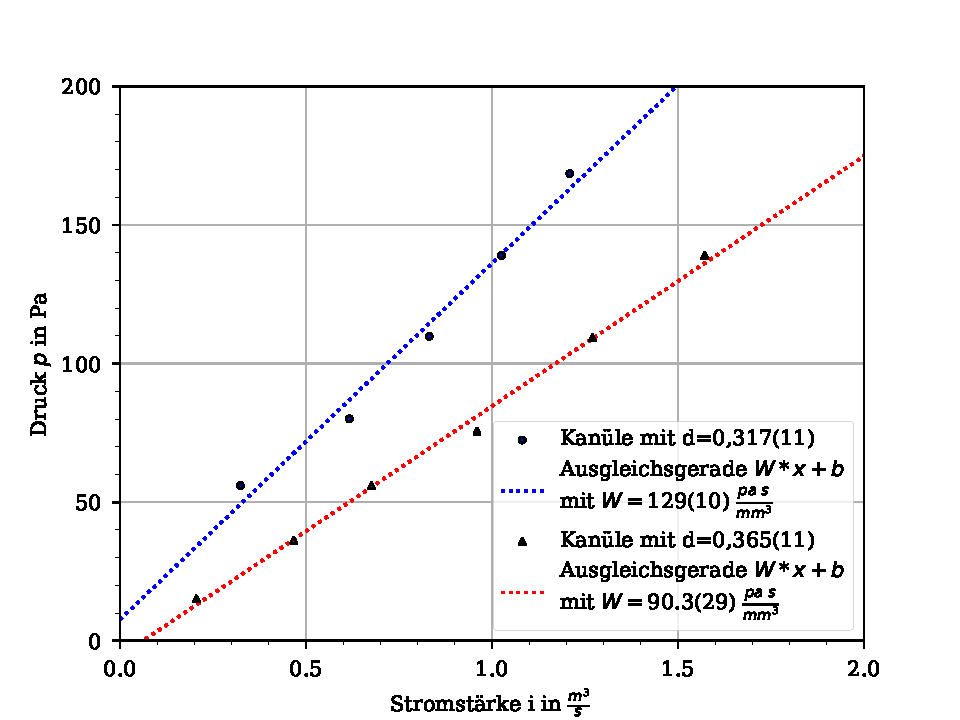
\includegraphics[width=\textwidth]{./1Plot.pdf}

        \caption{Messdaten, bestimmung des Strömungswiderstands}
        \label{fig:mess}
    \end{figure}
    In Graph \ref{fig:mess} wurde die gemessene Stromstärke gegen den anliegenden Wasserdruck aufgetragen.
    Die Strömungswiederstände $W_1 = 129(10) \si{\pascal\second\per\cubic\milli\metre}$ und 
    $W_2 = 90,3(29) \si{\pascal\second\per\cubic\milli\metre}$ wurden mithilfe einer gefitteten Ausgleichsgerade
    bestimmt. Aus den Messwerten in Tabelle \ref{tab:mess1} kann jetzt die dynamische Viskosität (Siehe \ref{tab:erg1}) von Wasser
    ausgerechnet werden.
    \begin{table}
        \centering
        \begin{tabular}{c c c}
            gemessene Größe & Kanüle 1 & Kanüle 2 \\ \hline
            Strömungswiderstand $W$ & $129(10) \si{\pascal\second\per\cubic\milli\metre}$ & $90,3(29) \si{\pascal\second\per\cubic\milli\metre}$ \\
            Länge $l$ & $31,05(10) \si{\milli\metre}$ & $31,55(10) \si{\milli\metre}$ \\
            Innendurchmesser $d$ & $0,315(10) \si{\milli\metre}$ & $0,365(10) \si{\milli\metre}$ \\
            
        \end{tabular}
        \caption{Messwerte Kapillarviskosimeter}
        \label{tab:mess2}
    \end{table}
    \begin{table}
        \centering
        \begin{tabular}{c}
            $\eta_1 = 0,00100(15) \si{\pascal \second}$ \\
            $\eta_2 = 0,00125(15) \si{\pascal \second} $ \\
            $\eta_g = 0,00113(13) \si{\pascal \second} $ \\
        \end{tabular}
        \caption{Ergibnisse dynamische Viskosität}
        \label{tab:erg1}
    \end{table}

    \subsection{Diskussion}
    Vergeicht man das Ergebnis mit dem Literaturwert $\eta_L = 1 \si{\pascal\second}$ \cite[Abb. 8]{VIS} bei einer Temperatur
    von $20 \si{\celsius}$ sieht man, dass der Literaturwert genau ein sigma Abstand zum Mittelwert hat.
    Schaut man sich die zwei verschiedenen Messreihen an, sieht man, dass die erste genau auf dem Literaturwert
    liegt. Die zweite Messreihe mit der blauen Kanüle weicht hingegen deutlich vom Theoriewert ab.
    Vermutlich liegt dies an einem Messfehler des Gewichts, Längen-
    oder Durchmesserbestimmung. 



    \section{Anhang}
    \subsection{Kugelfallviskosimeter}

    \subsubsection{Berechnung der dynamischen Viskosität mit Fehler} \label{sec:dynvisc}
    
    \begin{table}
       \begin{adjustwidth}{-5cm}{-5cm}
            \centering
            \begin{tabular}{c c c}
                Messgröße & Messwert mit Fehler & Begründung \\ \hline
                
                Gewicht $m$ & $g = 0,8445(5) \si{\gram}$ & Skalierung \\
                Durchmesser Kugel $d$ & $d = 3,998(17) \si{\milli\meter}$ & Student-t \\
                Durchmesser Zylinder $D$ & $D = 5,33(6) \si{\milli\meter}$ & ABW Skript \cite[Tabelle 6]{ABW} \\
                Zeit $t$ & $t = 3,85(15) \si{\second}$ & Reaktionszeit x2\\
                Strecke $s$ & $s = 35,00(21) \si{\milli\metre}$ & Schrittweite $1 \si{\milli\metre}$ \\
                Dichte Flüssigkeit $\rho_F$ & $\rho_F = 1,2220(21)  \si{\gram\per\milli\litre}$ & Schrittweite $0,01 \si{\kilogram\per\cubic\metre}$ \\

            \end{tabular}
        \end{adjustwidth}
        \label{tab:errors}
        \caption[]{Fehler der Messgrößen}
    \end{table}
    
    Als erstes wurde der Mittelwert der Fallzeiten berechnet.
    \begin{align}
        \bar{t} &= \frac{1}{n} \sum_{i=1}^{n} t_i = 3,94(15) \si{\second}
    \end{align}
    Der Fehler der Fallzeiten wurde mithilfe der Student-t-Verteilung (n=10) berechnet.
    \begin{align}
        u_{\bar{t}} &= \frac{{\it t}}{\sqrt{n}} u_{t_i} =  0,144 \si{\second}
    \end{align}
    Auch vom Kugeldurchmesser kann erstmal der Mittelwert
    \begin{align}
        \bar{d} &= \frac{1}{n} \sum_{i=1}^{n} d_i = 3,998(17) \si{\milli\metre}
    \end{align}
    und dann der Fehler mit Student-t (n=10)
    \begin{align}
        u_{\bar{d}} &= \frac{{\it t}}{\sqrt{n}} u_{d_i} = 0.017 \si{\milli\metre}
    \end{align}
    berechnet werden

    Jetzt kann $\eta$ mit Formel \cite[(11)]{VIS}
    \begin{align}
        \eta &= \frac{2r^2g}{9v}(\rho_K - \rho_F)  \nonumber \\
        &= \frac{2\frac{d}{2}^2g}{9\frac{s}{\bar{t}}}(\frac{m}{\frac{4}{3} \pi \frac{d}{2}^3} - \rho_F) \nonumber \\
        &= 0,1244(51) \si{\pascal\second}
    \end{align}
    und der Fehler mit der Gausschen Fehlerfortpflanzung \cite{ABW}
    \begin{align}
        u_{\eta} &= \sqrt{\sum^5_{i = 1}\left(\frac{\partial \eta}{\partial x_i}\right)^2 u_i^2} \\
        &= \frac{\sqrt{\frac{g^{2} \cdot \left(16 \pi^{2} r^{8} s^{2} t^{2} u_{\rho}^{2} + r^{2} s^{2} \cdot \left(9 t^{2} u_{m}^{2} + u_{t}^{2} \left(3 m - 4 \pi r^{3} \rho_{f}\right)^{2}\right) + r^{2} t^{2} u_{s}^{2} \left(3 m - 4 \pi r^{3} \rho_{f}\right)^{2} + s^{2} t^{2} u_{r}^{2} \left(3 m + 8 \pi r^{3} \rho_{f}\right)^{2}\right)}{r^{4} s^{4}}}}{18 \pi} \\
        &= 0,0051 \si{\pascal\second}
    \end{align}
    ausgerechnet werden.
    Mit der Formel \cite[(12)]{VIS} kann
    \begin{align}
        \eta = 0,1054(44) \si{\pascal\second}
    \end{align}
    sogar noch genauer ausgerechnet werden.
    \subsubsection{Berechnung der Reynoldszahl mit Fehler} \label{sec:reynolds}
    Mit der dynamischen Viskosität $\eta$ kann die Reynoldszahl $Re$ berechnet werden.
    \begin{align}
        Re &= \frac{\frac{d}{2} \rho_F v}{\eta} \nonumber \\
            &= 2,11(17)
    \end{align}
    Als charakteristische Länge wurde der Radius $r$ der Kugel benutzt, aber auch mit Durchmesser
    wäre die Reynoldszahl größer als 1.
    \subsection{Frage}
    \subsubsection{Fallschirmspringer}
    Annahmen: Fallschirmspringer ist eine Kugel mit Radius $r = 0,4 - 0,8 \si{\metre}$ und Masse $m = 80 \si{\kilogram}$, Luftdichte bei ca. 2000m $rho_F = 1 \si{\kilogram\per\cubic\metre}$.
    Damit kann die Viskosität der Luft
    \begin{align}
        \eta &= \frac{2 r^2 g}{9 v}(\frac{3m}{4 \pi r^3} - \rho_F) \nonumber \\
        &= 0,9 - 1,9 \si{\pascal\second}
    \end{align}
    und die Reynoldszahl
    \begin{align}
        Re &= 11 - 50
    \end{align}
    berechnet werden. Es treten in jedem Fall turbulente Strömungen auf. Die Annahmen sind nicht optimal, da ein Fallschirmspringer je nach Körperhaltung (Ausgestreckt oder als Kugel)
    sehr unterschiedliche Reibung hat und damit unterschiedliche Geschwindigkeiten erreichen kann. Es wurde aber nicht angegeben, mit welcher Körperhaltung
    er $200 \si{\kilo\metre\per\hour}$  schnell fällt, so können je nach Annahme verschiedene Viskositäten berechnet werden.
    Außerdem sind diese Werte verglichen mit Literaturwerten ($18 \si{\micro\pascal\second}$)falsch, da vermutlich die Reibung der Luft mit turbulenten Strömungen
    nicht mit der verwendeten Stokesschen Formel \cite[(9)]{VIS} berechnet werden kann.

    \subsubsection{Atmung}
    Annahmen: Radius Nasenloch $r = 3 \si{\milli\metre}$,  Viskosität der Luft $\eta = 18 \si{\micro\pascal\second}$,
    Atemfrequenz $f = 0,25 \si{\hertz}$. Daraus folgt, dass ein Einatmen genau zwei Sekunden dauert.
    \begin{align}
        v &= \frac{V}{\pi r ^2 \cdot t} \nonumber \\
            &= 8.84 \si{\metre\per\second}
    \end{align}
    Mit der Geschwindigkeit kann man die Reynoldszahl
    \begin{align}
        Re &= \frac{2r \rho_F v}{\eta} \nonumber \\
        &= 3802
    \end{align}
    berechnen. Da diese größer als 2300 ist, entstehen Verwirbelungen.
	Bei verstärkter Atmung mit einem Volumen von $V = 1 \si{\litre} = 0,001 \si{\metre\cubed}$
	ist die Luft noch turbulenter mit Reynoldszahl von $Re &= 7604$
    \bibliographystyle{plain}
    \bibliography{literature}

\end{document}